\chapter{STATE OF THE ART: A RAPID REVIEW ON CLOUD-NATIVE OBSERVABILITY}
\label{chap:related-work}

As detailed in Chapter \ref{chap:observability} and illustrated in Figure \ref{fig:cna-obs-evo}, the landscape of cloud-native observability has undergone significant evolution over the years. While numerous tools have been developed to tackle isolated observability concerns, there is a distinct lack of cohesive efforts to unify them into a comprehensive architecture. The most mature initiative to date is driven by the Cloud Native Computing Foundation (CNCF) \cite{cncf_2026}, which accepted the OpenTelemetry project in 2019 and formally promoted it to a graduated maturity level in 2026.

\begin{figure}[ht]
    \centering
    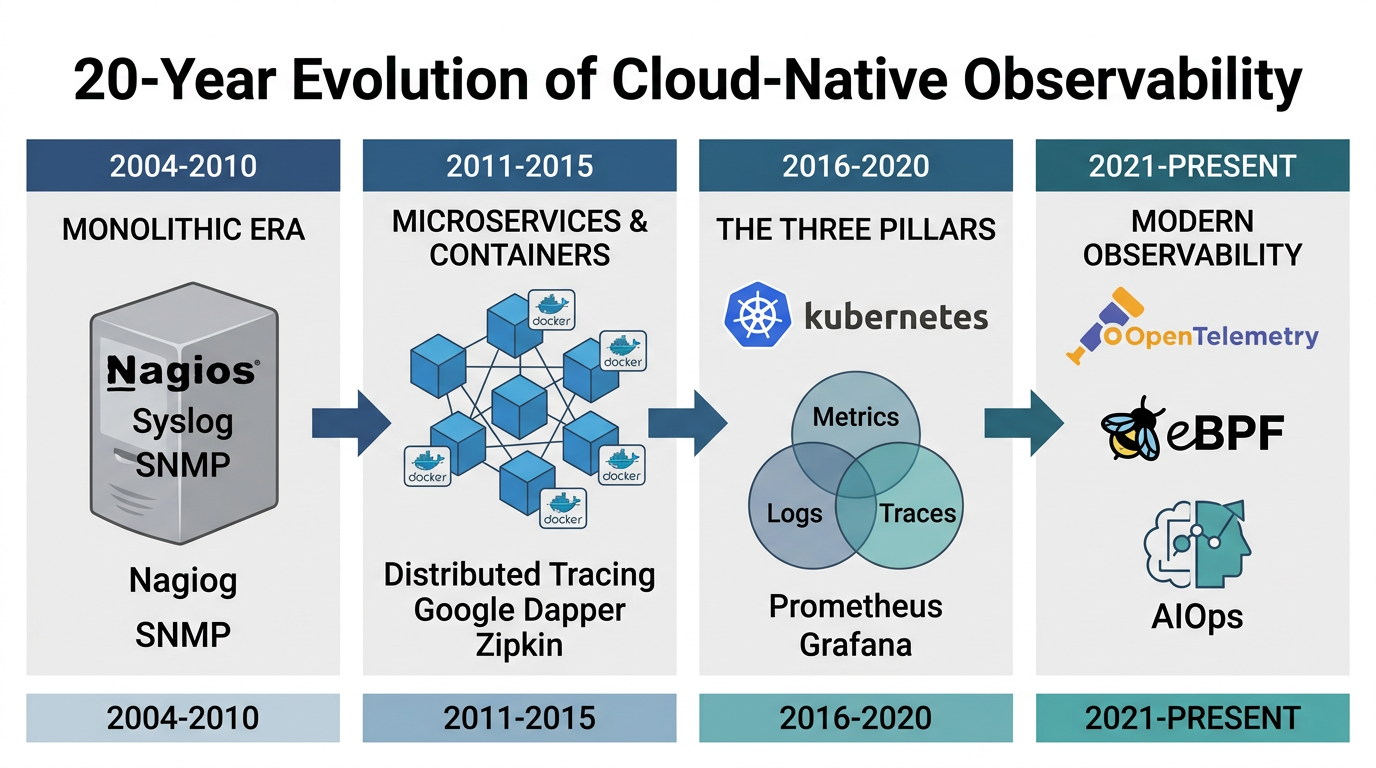
\includegraphics[width=1.0\linewidth]{images/observability/cloud_native_observability_evolution.png}
    \caption{Cloud Native Observability Evolution}
    \label{fig:cna-obs-evo}
\end{figure}

To understand this panoram and ensure the scientific rigor required for a doctoral thesis and to systematically map the solution space regarding cloud-native observability, a Rapid Review (RR) of the literature was conducted. 

Unlike traditional ad-hoc literature reviews, a Rapid Review provides a structured, replicable protocol to synthesize evidence promptly without compromising systematic rigor \cite{cartaxo_2018}. By mapping the state of the art, this chapter identifies the exact boundaries of current open-source implementations and theoretically justifies the architectural gaps that this thesis aims to bridge.

This chapter details the methodology applied, analyzes the primary studies identified across four major scientific databases, proposes an Observability Maturity Model (OMM) based on the identified gaps, and explicitly positions the proposed PANOPTES architecture within the current research landscape.

\section{Rapid Review}
\label{sec:rapid-review}

To map how the industry and academia are addressing this analytical shift in Kubernetes-based environments, we conducted a Rapid Review. Rapid Reviews are secondary studies designed to provide timely research evidence to support decision-making in practical environments, offering a structured approach without the exhaustive timeline of a full Systematic Literature Review \cite{cartaxo_2018}.

\subsection{Rapid Review Protocol}

Rapid Reviews (RRs) are secondary studies designed to provide timely research evidence to support decision-making in practical environments \cite{cartaxo_2018}. RRs are conducted considering constraints inherent to practical environments, such as time and effort, thus delivering evidence more promptly and at lower costs, often communicated through accessible mediums.

This approach is particularly suitable for our study, as it aims to swiftly synthesize scientific evidence on the rapidly evolving field of observability in cloud-native applications without compromising systematic rigor. An RR complements Systematic Reviews (SRs) by filling an essential gap in promoting evidence-based, practice-oriented software engineering for urgent research questions.

Similar to SRs, this Rapid Review consisted of three main phases: planning, performing, and reporting. These phases are detailed in the following subsections.

The execution of this Rapid Review, initially published as an independent study \cite{silva_2026}, served as the foundational investigative step for this thesis. It is imperative to highlight the structural alignment between the research questions of this review (RQ01--RQ04) and the Secondary Research Questions (SRQ) of this doctoral research:

\begin{itemize}
    \item \textbf{Theoretical Foundation (RQ01 and RQ03 $\rightarrow$ SRQ1):} The investigation into essential components (RQ01) and specific open-source tools (RQ03) provided the necessary literature backing to answer the thesis's SRQ1, effectively defining the required technological stack (Metrics, Logs, and Traces via CNCF tools) for the experimental environment.
    \item \textbf{Gap Identification and Modeling (RQ02 and RQ04 $\rightarrow$ SRQ4):} The search for existing reference architectures (RQ02) and the subsequent identification of fragmentation gaps (RQ04) directly addressed the thesis's SRQ4. The realization that the industry lacks a unified framework culminated in the proposition of the Observability Maturity Model (OMM).
\end{itemize}

Ultimately, while this Rapid Review answers the theoretical constraints of the domain, it acts as the springboard for the practical contributions of this thesis (SRQ2 and SRQ3)—specifically, the instantiation of the PANOPTES architecture and its empirical validation.

\subsection{Planning Phase}
In the planning phase, we followed a detailed protocol for this Rapid Review, as established by Cartaxo \textit{et al.} \cite{cartaxo_2018}. This protocol encompassed the formulation of the research problem, the specific research questions (RQs), the search strategy, the selection criteria, and the data extraction procedure. The online tool Parsifal was utilized to systematically compile and manage all aspects of this protocol, ensuring transparency and adherence to a predefined methodology.

Cloud-native environments, characterized by microservices, containers, and dynamic orchestration (e.g., Kubernetes), inherently generate an exponentially growing volume, variety, and velocity of telemetry data (logs, metrics, traces, and events). Managing, processing, and storing this vast amount of raw data becomes economically prohibitive and technically unfeasible. As highlighted by \cite{sridharan_2018}, this exponential growth in data significantly constrains a system's capacity to process information and to deal effectively with ``unknown unknowns,'' necessitating robust observability solutions.

\subsection{Research Questions}
The goal of this study is to identify the state of the art in observability of Kubernetes-based cloud-native applications and investigate the open-source tools and architectural patterns deployed to achieve the degree of observability proposed in the literature. To guide this Rapid Review, the following research questions were formulated:

\begin{itemize}
    \item \textbf{RQ01:} What are the essential components of an observability architecture for Kubernetes-based cloud-native applications?
    \item \textbf{RQ02:} What reference architectures or observability frameworks for Kubernetes-based cloud-native environments have been proposed in the literature?
    \item \textbf{RQ03:} What open-source tools are used or recommended to implement the different components of a Kubernetes-based observability architecture for cloud-native applications?
    \item \textbf{RQ04:} What research gaps and future directions have been identified in the literature on open-source observability architectures for Kubernetes-based cloud-native applications?
\end{itemize}

\subsection{Performing Phase}
The performing phase involved the systematic execution of the search and study selection procedures as defined in the planning phase. The literature search was primarily conducted using four leading scientific databases known for their extensive coverage in Computer Science and Software Engineering: IEEE Xplore, ACM Digital Library, SpringerLink, and ScienceDirect. These databases were selected for their relevance to cloud computing, distributed systems, and software observability. The temporal scope of the search was set from January 2018 to October 2025, with a focus on recent developments in the field.

The search string, carefully constructed and adapted for each database's specific syntax using the filter full-text, was:

\begin{quote}
\textbf{Search String:} (``cloud native" OR ``cloud-native'' OR ``microservices") AND (``observability'' OR ``monitoring'' OR ``tracing'' OR ``logging'' OR ``metrics'' OR ``events'') AND (``kubernetes" OR ``k8s'') AND (``open source" OR ``open-source'')
\end{quote}

Initial searches identified seminal works such as \cite{kosinska_2023} and \cite{usman_2022}, which served as starting points for a complementary forward and backward citation analysis to identify additional relevant studies. Furthermore, an AI-powered literature discovery tool (Research Rabbit) was used to expand the literature search through intelligent recommendation algorithms, efficiently identifying related works and emerging topics based on the initial relevant papers.

The identified studies underwent a multi-stage selection process based on predefined Inclusion and Exclusion Criteria. The study selection process consists of three distinct stages: initial screening, full-text review, and conflict resolution. Initially, titles and abstracts were reviewed by a single researcher to assess their potential relevance. In the second stage, studies that passed the initial screening proceeded to full-text review to confirm their direct relevance to the research questions and ensure full compliance with all criteria. In the third case, when uncertainty or disagreement arose during the full-text review, a second researcher was consulted to resolve conflicts and make a final decision on inclusion.

Six inclusion criteria (IC) were used: \textbf{IC01} - Primary focus on Observability for software systems; \textbf{IC02} - Context related to cloud-native applications or microservices; \textbf{IC03} - Discussion of Kubernetes as the orchestration platform; \textbf{IC04} - Focus on open-source observability tools or architectures; \textbf{IC05} - Articles published from January 2018 to October 2025; \textbf{IC06} - Articles written in English.

Similarly, six exclusion criteria (EC) were used: \textbf{EC01} - Duplicated papers; \textbf{EC02} - Gray literature (e.g., blog posts, pre-prints without peer review, company whitepapers); \textbf{EC03} - Focus exclusively on monitoring without addressing observability concepts; \textbf{EC04} - Studies where observability is only tangentially mentioned or not a primary contribution; \textbf{EC05} - Articles exclusively discussing proprietary or closed-source solutions without comparison to open-source alternatives; \textbf{EC06} - Books, book chapters, theses, dissertations, and short papers (e.g., extended abstracts, posters).

For each selected study, data relevant to the research questions were systematically extracted by one researcher and validated by another using the Parsifal online tool. The following information was collected: \textbf{for RQ01:} Definitions of essential architectural components, layers of observability (e.g., data types, functional capabilities, instrumentation levels). \textbf{For RQ02}, descriptions of proposed architectural patterns, frameworks, or significant architectural considerations. \textbf{For RQ03}, the identification of specific open-source tools, their functionalities, and their application within Kubernetes-based environments. Finally, \textbf{for RQ04}, identified research challenges, gaps, and future directions related to open-source observability. This structured approach ensured consistency and scientific rigor in the data collection process.

\subsection{Findings and Architectural Gaps}

The rapid review revealed critical insights into the current landscape of cloud-native observability. Table \ref{tab:related_works} summarizes the primary studies analyzed and their respective identified gaps and proposed future works.

\begin{table*}[!ht]
\centering
\caption{Analysis of Related Works and Primary Studies Cited}
\label{tab:related_works}
\footnotesize
% As larguras somam ~0.91\textwidth, deixando espaço para o padding (tabcolsep)
\begin{tabular}{p{0.15\textwidth} p{0.38\textwidth} p{0.38\textwidth}}
\toprule
\textbf{Ref.} & \textbf{Research Gaps and Limitations found} & \textbf{Future Works} \\ \midrule

\cite{usman_2022} &
Absence of formal reference architecture, operational complexity of fragmentation, telemetry limitations, and scalability and correlation challenges. & 
Intelligent Automation via AI/ML, Security integration, Enhancing Developer Experience, and Unified Observability Platforms. \\ \addlinespace

\cite{araujo_2024} &
Lack of holistic reference architectures, resource constraints (overhead) in fog nodes, and high heterogeneity of edge devices. & 
Lightweight AI/ML for local anomaly detection (TinyML), standardized interoperability protocols, and adaptive observability frameworks. \\ \addlinespace

\cite{zanatta_23} &
Fragmented focus on metrics over logs/traces in 5G research, high memory/CPU overhead of standard CNOT stacks, and lack of standardized log structures. & 
Integration of distributed tracing, research on geographically distributed B5G setups, scalability analysis of COTS ML, and observability in Open RAN components. \\ \addlinespace

\cite{kosinska_2023} &
Lack of unified terminology, insufficient practical automation via AI/ML (AIOps gap), and poor adaptation of tools for edge computing environments. & 
Development of observability maturity models, deeper integration with eBPF for low-overhead visibility, and alignment with FinOps and GreenOps. \\ \addlinespace

\cite{faseeha_2025} &
Conceptual confusion between monitoring and observability pillars, lack of practical multi-pillar approaches, and difficulties in tracing failures in highly dynamic environments. & 
Evolution of frameworks for modern deployment paradigms (service mesh, event-driven), automation of data analysis, and optimization of observability overhead. \\ \addlinespace

\cite{han_2024} &
Inconsistent problem definitions for RCA and high cloud-native heterogeneity across traces, metrics, and logs. & 
Improving multi-modal data correlation at scale and enhancing Graph Attention Networks for dynamic topologies. \\ \addlinespace

\cite{gomes_2025} &
Difficulty in correlating multi-modal data (metrics, logs, traces), inadequacy of traditional monitoring for sophisticated CNAs, and complex root cause analysis (RCA) in distributed environments. & 
Advanced ML-based resource management, automated diagnostic mechanisms integrated with auto-scaling, and research on low-overhead real-time data collection. \\ \addlinespace

Wei et al. \cite{wei_2025} &
Lack of a systematic bridge between desirable system qualities and the concrete cloud-native practices and tools used to achieve them, and the initial validation scope is limited (expert-based, not covering all contexts). &
Provide mechanisms/interfaces to extend and continuously evolve the map (keeping practices/tools up to date) and perform broader validations beyond the initial expert review. \\ \addlinespace

\cite{deng_2024} &
Missing clear research roadmap for cloud-native lifecycles, high cognitive load for developers (DevEx), and insufficient real-time security observability. & 
Integration of SecOps with performance telemetry, improvement of Developer Experience (DevEx), and observability optimization for serverless and green computing. \\ \bottomrule
\end{tabular}
  \par\medskip\ABNTEXfontereduzida\selectfont\textbf{Fonte:} Written by author (2026) \par\medskip
\end{table*}

A significant finding from this review is the scarcity of widely adopted, formal reference architectures specifically tailored for the dynamic nature of Kubernetes. While academic research has proposed structured life cycles \cite{araujo_2024}, there is a distinct lack of proposals that adequately manage the simultaneous collection and correlation of metrics, logs, and traces in an integrated manner without excessive overhead.

Instead, a ``de facto'' pattern has emerged driven by the integration of specific open-source tools. OpenTelemetry has become the industry standard for unified instrumentation \cite{kosinska_2023}. Meanwhile, specific tools dominate their respective pillars: Prometheus for metrics, Loki or Fluentd for logging, and Jaeger or Tempo for distributed tracing \cite{usman_2022}.

However, the literature unanimously warns that these tools are rarely ``plug-and-play''. This fragmentation imposes significant operational complexity on engineering teams, who must manually manage configurations and data correlation, highlighting the critical gap that the PANOPTES reference architecture proposed in this thesis aims to bridge.
\input{chapters/03.obs_related_work/sections/02_analysis_studies}
\section{The Observability Maturity Model (OMM)}
\label{sec:omm}

As a direct outcome of the Rapid Review conducted to address Specific Objective \textbf{SO4}, this research formalizes and proposes the \textit{Observability Maturity Model} (OMM). Maturity models are widely recognized in software engineering and IT service management as effective instruments for assessing organizational capabilities, diagnosing operational gaps, and guiding staged process improvements \cite{proenca_2016}. However, within the Information Systems (IS) literature, maturity models must not be treated as simple, ad-hoc checklists; rather, they represent complex, multi-dimensional **design artifacts** that require rigorous conceptual design, clear boundary definitions, and empirical validation \cite{mettler_2011}.

To establish a solid scientific foundation for the OMM, this research adopts a hybrid methodological framework combining the procedure design guidelines of \citeonline{becker_2009}, the design science research perspective of \citeonline{mettler_2011}, and the developmental lifecycle model of \citeonline{debruin_2005}.

\subsection{Methodological Design and Requirements Alignment}
According to \citeonline{becker_2009}, the development of a scientifically rigorous maturity model must satisfy eight fundamental design requirements to ensure its reliability and academic validity. Table \ref{tab:omm-becker-alignment} outlines how the OMM aligns with and satisfies each of these requirements.

\begin{table}[ht]
\centering
\footnotesize
\caption{OMM Alignment with Becker et al. (2009) Design Requirements}
\label{tab:omm-becker-alignment}
\begin{tabularx}{\textwidth}{|l|X|}
\hline
\textbf{Design Requirement} & \textbf{OMM Instantiation in this Thesis} \\ \hline
1. Comparison with existing models & Our literature synthesis (Chapter 3) mapped existing siloed APM/monitoring maturity models, highlighting the lack of cloud-native and correlation-focused frameworks. \\ \hline
2. Iterative research strategy & The OMM was refined cyclically across the design and prototyping phases of the PANOPTES architecture. \\ \hline
3. Evaluation & The model's target state (Level 4) is evaluated through a controlled experiment using Chaos Engineering (Chapter 7). \\ \hline
4. Multi-method presentation & Developed via a systematic literature synthesis (Rapid Review) and evaluated via quantitative systems engineering experiments. \\ \hline
5. Detailed documentation & All stages of the design, metric definitions, and evaluation scripts are fully documented and public. \\ \hline
6. Target audience definition & The model explicitly targets Site Reliability Engineers (SREs), system architects, and operations managers. \\ \hline
7. Problem definition & Addresses the complexity and fragmentation of telemetry data ($Metrics, Logs, Traces, Events$) in ephemeral Kubernetes environments. \\ \hline
8. Design results & Delivers a prescriptive framework capable of guiding organizations from siloed monitoring to unified, correlated observability. \\ \hline
\end{tabularx}
\par\medskip
\ABNTEXfontereduzida\selectfont\textbf{Source:} Developed by author (2026)
\end{table}

Furthermore, \citeonline{mettler_2011} argues that maturity models must be conceptualized as decision-support artifacts that assist managers in organizational design. By leveraging the three purposes of use defined by \citeonline{debruin_2005}, the OMM is structured to evolve through three distinct utilitarian stages:
\begin{itemize}
    \item \textbf{Descriptive Utility:} Act as a diagnostic tool to assess the current "as-is" state of a Kubernetes cluster's telemetry pipelines, isolating unindexed logs and missing distributed traces.
    \item \textbf{Prescriptive Utility:} Provides a clear, actionable evolutionary roadmap. The PANOPTES reference architecture acts as the prescriptive engineering vehicle designed to elevate a cluster from lower levels to Level 4 (Optimized).
    \item \textbf{Comparative Utility:} Enables future benchmarking by allowing organizations to compare their diagnostic efficiency ($MTTDiag$) against the resource overhead footprint ($CPU/Memory$), establishing comparative trade-offs.
\end{itemize}

\subsection{The Development Phases of OMM and the Validation Gap}
To construct and validate the model, this work follows the six-stage developmental framework proposed by \citeonline{debruin_2005}. Figure \ref{fig:model-dev-phases} illustrates this lifecycle, which we operationalize as follows:

\begin{figure}[ht]
    \centering
    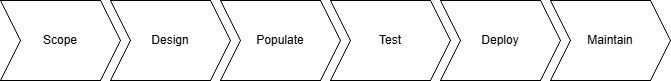
\includegraphics[width=1.0\linewidth]{images/observability/model-development-phases.png}
    \caption{Maturity Model Development Lifecycle (De Bruin et al., 2005)}
    \label{fig:model-dev-phases}
    \par\medskip\ABNTEXfontereduzida\selectfont\textbf{Source:} \citeonline{debruin_2005} \par\medskip
\end{figure}

\begin{itemize}
    \item \textbf{Scope:} Defined as a domain-specific model focusing exclusively on cloud-native containerized applications orchestrated by Kubernetes, addressing the architectural gaps in correlating multi-signal telemetry data.
    
    \item \textbf{Design:} Employs a multi-dimensional, stage-based linear architecture. It defines the telemetry space mathematically as the set $O = \{M, L, T, E\}$—representing Metrics, Logs, Traces, and Events, respectively—and evaluates capability across three layers: ingestion, storage correlation, and diagnostic retrieval.
    
    \item \textbf{Populate:} Achieved through a hybrid approach combining top-down stage definitions with a bottom-up population of capabilities, synthesized from the 237 primary studies identified in the Rapid Review.
    
    \item \textbf{Test (Mitigating the Validation Gap):} In a seminal systematic mapping study, \citeonline{wendler_2012} analyzed 237 maturity model publications and identified a critical research gap: **the Validation Gap**. The vast majority of academe-designed maturity models are published with speculative, qualitative evaluations (e.g., self-assertions or unvalidated case studies), lacking empirical, repeatable, and quantitative validation of their target states. 
    
    Our research directly mitigates this Validation Gap. We subject the model's target state (\textbf{Level 4 - Optimized}) to an exhaustive, automated, and controlled system-level experiment (Chapter 6 \& 7). By executing $N=30$ runs under randomized chaos (using Chaos Mesh), we provide empirical, statistically sound proof (using Mann-Whitney U testing) that transitioning to Level 4 capabilities reduces the Mean Time to Diagnose ($MTTDiag$) without violating resource bounds.
    
    \item \textbf{Deploy:} Instantiated and shared with the research and DevOps communities as reproducible open-source Infrastructure as Code artifacts (Multipass, Ansible, and Helm charts), enabling immediate replication and adoption.
    
    \item \textbf{Maintain:} Designed with an open capability architecture that anticipates technological evolution. It establishes Level 4 as the necessary data substrate required to support Level 5 (Predictive) AIOps models, which cannot function without correlated, high-fidelity traces and logs.
\end{itemize}

\subsection{OMM Evolutionary Levels}
As a result of the \textit{Scope}, \textit{Design}, and \textit{Populate} phases, we formalize the OMM across five cumulative levels of maturity, mapping the operational state of the telemetry set $O = \{M, L, T, E\}$:

\begin{enumerate}
    \item \textbf{Level 1 - Non-Existent:} The system is a complete black box. Telemetry data $O = \emptyset$. No logs, traces, or metrics are systematically collected. Troubleshooting is purely reactive, relying on user complaints and manual container restarts.
    
    \item \textbf{Level 2 - Initial/Ad-Hoc:} Characterized by siloed and fragmented telemetry ($O = \{M_{\text{local}}, L_{\text{local}}\}$). Metrics and container logs are scraped on-demand or stored locally within ephemeral nodes. Distributed traces are completely absent ($T = \emptyset$). Isolating cascading failures requires unindexed manual log searching, causing high cognitive load and long, non-deterministic diagnostic cycles.
    
    \item \textbf{Level 3 - Managed (Centralized):} Centralized collection is established ($O = \{M_{\text{central}}, L_{\text{central}}, T_{\text{siloed}}\}$). A telemetry collector aggregates data into distinct storage backends (e.g., separate databases for logs, metrics, and traces). While data is centralized, the signals remain un-correlated. Site Reliability Engineers (SREs) must manually pivot between different visualization tools or copy-paste trace IDs to correlate anomalies.
    
    \item \textbf{Level 4 - Optimized (Correlated - The PANOPTES Target):} Fully correlated, multi-modal telemetry is operationalized ($O = \{M \bowtie L \bowtie T \bowtie E\}$). The telemetry pipeline enforces strict semantic binding, linking metrics to traces using exemplars, and traces to logs using contextual span metadata. SREs navigate a single pane of glass, accelerating fault isolation. The empirical validity of this stage's diagnostic superiority is the core contribution of this thesis.
    
    \item \textbf{Level 5 - Predictive (AIOps):} Telemetry streams feed autonomous, intelligent closed-loop control agents ($O = f(M, L, T, E) \rightarrow \text{Control Action}$). Machine learning, variational autoencoders, and causal inference models ingest the high-fidelity correlated datasets provided by Level 4 to predict anomalies, execute auto-remediation, and dynamically scale resources before failure cascades impact end-users.
\end{enumerate}

By formalizing these evolutionary stages, the OMM provides a clear, scientifically grounded roadmap that helps researchers and practitioners navigate the complex landscape of cloud-native systems, positioning the PANOPTES architecture as the structural bridge to high-maturity operations.
\input{chapters/03.obs_related_work/sections/04_panoptes_positioning}